\documentclass [11pt, proquest] {uwthesis}[2020/02/24]
\usepackage{graphicx}
\graphicspath{ {./images/} }

\setcounter{tocdepth}{1}  % Print the chapter and sections to the toc

\let\mffont=\sf

\begin{document}

\prelimpages

\Title{Securing WireGuard private keys with a hardware token\\}
\Author{Peter Van Eenoo}
\Year{2022}
\Program{Computer Science and Engineering}

\Chair{Brent Lagesse}{Dr.}{Computing \& Software Systems}
\Signature{William Erdly}
\Signature{Yang Peng}

\copyrightpage

\titlepage  


\setcounter{page}{-1}
\abstract{





%\footnote{See Appendix A to obtain the source to this
% thesis and the class file.}
}

%
% ----- contents & etc.
%
\tableofcontents
\listoffigures

\chapter*{Glossary}      % starred form omits the `chapter x'
\addcontentsline{toc}{chapter}{Glossary}
\thispagestyle{plain}

\begin{glossary}

\item[WireGuard]

a VPN technology created in 2017 by Jason DonenFeld that operates at the network layer, which aims to replace popular TLS-based VPNs like OpenVPN and IPsec.
WireGuard has been described as “crypto-opinionated”, meaning the WireGuard protocol supports only one cryptographic primitive for each cryptographic requirement.
There is no support for negotiation of cryptographic parameters. For example, WireGuard only supports ChaCha20 for symmetric 
encryption\cite{donenfeld_wireguard_2017} of data and Curve25519 key pairs for client authentication and key exchange.

\item[Curve25519]
an elliptic curve with a keys size of 256 bits designed by Daniel J. Bernstein in 2005\cite{noauthor_curve25519_nodate}. Key-s operations are referred to as . 
This distinction is important because WireGuard uses only X25519 operations for  key exchange, 
when generating the ephemeral session keys.

\item[X25519]
a key exchange algorithm that uses Curve25519 to implement Elliptic-curve Diffie–Hellman (ECDH) key exchange. This process is also known as key derivation function (KDF).

\item[Ed25519] a digital signature algorithm that uses the Curve25519.

\item[PKCS\#11] a public-key cryptography standard governed by the OASIS technical committee\cite{noauthor_cryptsoft_nodate} that defines a common interface for programs that need to interact with security keys, also referred to as cryptographic tokens.

\item[Hardware security module]
(HSM) a dedicated, physical hardware device that safeguards digital keys and provides limited-access to the resident keys for operations such as but not limited to encryption, decryption, verification and authentication. 

\item[Security Key]
a general term for a class of devices that implement a limited subset of HSM functionality that securely store cryptographic keys and restricts access through a limited interface. These devices typically connect to a computer or smartphone via USB or NFC and are small enough to be held on a user's key-ring.
Nitrokey Start\cite{noauthor_nitrokey_nodate} or YubiKey\cite{noauthor_discover_nodate}\cite{noauthor_u2f_nodate-1} are examples of such devices.


\end{glossary}

\textpages

\chapter {Introduction}
WireGuard is a new implementation of a Virtual Private Network (VPN) proposed in 2017. A key design feature of WireGuard is the elimination of cryptographic algorithm negotiation between parties and instead, the protocol relies on a fixed-choices for cryptographic primitives. This greatly simplifies the design, implementation and attack surface of the protocol. Another design simplification that WireGuard uses is the management of public and private keys. WireGuard does not use x509 certificates or the traditional PKI infrastructure, instead each parties identity is a 256-bit curve25519-based public key. This public key is referred to as the static public key because it doesn't expire and is the starting point from which ephemeral public keys for every session are generated. The static public keys of the initiator and responder must be pre-shared with both parties respectively, before a successful handshake can be made. 

(TODO: talk about cookie back off mechanism) and uses a novel cookie mechanism with scaling-back-off, built into every implementation, in order to resist DDoS attacks. (RE-WORK SECTION LATER)

A benefit to the pre-shared static public key requirement, is that any party running WireGuard is resistant to active network enumeration. In order to get a response from a peer, the initiator's message must have knowledge of the responder's public key to get a response packet. 

WireGuard traffic is (TODO: talk about un-encrypted network traffic, it can be see but only 4 types)

The WireGuard VPN has had a successful mainstream adoption, as evidenced by its recent inclusion in many 
open-source operating systems\cite{donenfeld_wireguard_nodate} as well as a recent native Windows kernel module\cite{noauthor_wireguard-nt_nodate}. MacOS, IOS, Android, FreeBSD and OpenBSD are supported as well.



\section {Background}


\section {Contributions}
The Elliptic Curve, Curve25519 is being used in an increasing number of open-source and commercial products\cite{noauthor_things_nodate-1} from SSH to Signal, however hardware support in 
security keys is currently almost non-existent. YubiKey is currently the most popular security key manufacturer however all of their current products 
lack support for X25519. I hope my project, as the first open source project to combine an X25519 supported security key with a popular open source VPN like WireGuard, will encourage more manufactures to add support for X25519 across the security key industry.

\section {Related-work}
The WireGuard handshake protocol has gone through extensive formal verification using Tamarin proof system \cite{donenfeld_formal_2018}. Researchers have identified some potential weaknesses in WireGuard around quantum computers but no critical or serious vulnerabilities have been identified sine it was introduced five years ago in 2017.

The WireGuard protocol and handshake has been analyzed and dissected without any major flaws being yet discovered. Researchers have demonstrated vulnerabilities might exist for guarantees like perfect-forward-secrecy, if quantum computers can be used to break XXX.  In the area of post-quantum security, a redesign of WireGuard's handshake has been proposed by \cite{hulsing_post-quantum_2021}.
(TODO: ADD IN MORE BG INFORMATION FROM ONE-DRIVE PAPERS AND ADD A BETTER SUMMARY)

\section {WireGuard Handshake}
\ It will be necessary to understand the context that the private key is used in and how the WireGuard handshake authenticates clients, when we discuss our threat model in section~\ref{section:tm}. Next I will discuss some of the features of Curve25519 and it's place in WireGuard.
\subsection{Curve25519 public/private key pairs}
A feature of Curve25519 is that any 32-byte value is a valid private key and unlike some other elliptic curves, Curve25519 requires no key validation, to avoid small subgroup attacks, and is immune to some classes of timing attacks\cite{noauthor_safecurves_2022}\cite{sasdrich_implementing_2015}.  Deriving the public key from the private key is fast enough that programs such as WireGuard don't need to store the client's public key in in the configuration file and stores only the private key. When WireGuard starts, it reads it reads the saved private key and derives the public key. 

\section {Identity and handshake initiation}
\label{handshake_message}

\begin{figure}[ht]
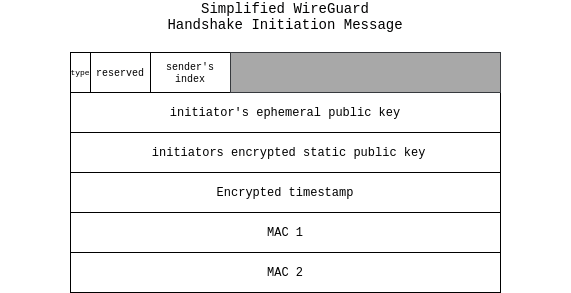
\includegraphics[width=12cm]{paper/images/Wg_hand_init.drawio.png}
\caption{simplified WireGuard handshake initiation message}
\label{fig:hand_init}
\end{figure}
In the WireGuard protocol, both parties are identified by their static public key's. WireGuard refers to parties as an initiator and a responder, since there is no strict definition of client or server. WireGuard assumes that each parties public key is securely exchanged out-of-band. This exchange must take place before a handshake can be performed. A handshake is performed using an initiation message, sent by the initiator to the responder. The most important fields in the handshake message are shown in Figure \ref{fig:hand_init}.

To create an initiation message, the initiator generates an ephemeral, Curve25519 key-pair The 32-byte ephemeral public key is added to the message. The initiator's static public key is encrypted using 
The sender's index is a randomly generated 4-byte value. It is used as a peer's chosen handshake session id.
The responder's public key used as key to MAC 1. This initiation message contains an encrypted form of the initiator's public key

The contents of the initiation message are authenticated using MAC 1.
A MAC is used to protect the initiation message, with the MAC key being the responders public key.

responder, an initiator is identified by their ability to decrypt messages encrypted with the client's public key, and cannot be revoked, except by manually notifying and removing the client’s public key from all servers. As mentioned previously, in WireGuard, key management is intentionally left up to the users and administrators. There is no certificate revocation mechanism or expiration of client and server keys.

TODO: timestamp description

MAC2 is an optional MAC and is used only when the anti-DDoS mechanism is enabled for a given responder. 

\section{compatibility}
Compatibility is an important area of consideration when modifying WireGuard. Since WireGuard has no negotiation of cryptographic primitives, any project that modifies the underlying cryptographic functions or protocol, will introduce client incompatibility and be restricted to working with only themselves. I designed WireGuard-HSM with this in mind. My goal was to improve the security of the current protocol while not introducing any client-incompatibility. This is verified by the ability of WireGuard-HSM to perform a successful handshake and pass traffic with unmodified peers.


\chapter {Project Background}

\section {Conception}
I was interested in WireGuard when it was announced but it wasn't until a group project I started in Winter 2020, where we looked at the security of WireGuard and primarily identified key handling as a potential weak point in the program, that I began to consider different approaches to improving WireGuard,  without introducing a larger attack surface or forking the project. 

In Spring quarter of 2021, I took research methods in software development with Dr Erdly. During this course I continued to explore ideas that I had about WireGuard and it's private key handling. I created my final project around WireGuard. In the project, I asked the question, how could WireGuard's private key handling be better? What systems could I create to improve it, and then how could I evaluate those systems?  
In the final part of the project I create a mock survey of software engineers to rate four of the final designs. I used my own metrics to define my terms (TODO finsh up this back story, get to point about compatibility)

I came up with three designs that would improve key handling in WireGuard and I rated them on implementation, TODO(dig up project and look at ratings)!! In the end I chose the simplest overall design with the biggest risk being that my design relied on a security key produced by a single manufacture. No other manufactuer at the time was making a security key that supported X25519.

\section{starting out}

I decided to start with interfacing with the NitroKey and getting familiar with the tools and commands to interact with it. I initially chose the Nitrokey start because it's product page said it supported X25519\cite{noauthor_nitrokey_nodate} which is the ECDH key derivation process. After a few frustrating days I couldn't figure out how to even generate or put a curve25519 key on the nitrokey start. Searching online, I didn't see any existing software projects that interfaced with a security key for performing X25519 operations. What I did discover after pouring over NitroKey's documentation was that they recommended using a program called OpenSC to work with the Nitrokey but that only a program called GnuPG, when running in an advanced configuration mode, was capable of telling the Nitrokey to generate a set of curve25519 keys. Confusingly, GnuPG can generate the correct keys but it has no ability to perform X25519 with the security key.

\section {OpenSC}
Key derivation for ECDH, called X25519 in my specific case when using Curve25519 keys, requires access to Bob's private key and Alice's public key. The cryptographic operation will generate a new 'shared key' that is identical for both parties when the keys are flipped and you use Alice's private key and Bob's public key. 
After researching the OpenSC tool support forums, I was able to find the command string that instructs a  security key to perform the key derivation operation with the correct inputs and outputs. However the tool only produced an error when I tried to use it with the Nitrokey and Alice's public key. I discovered that while NitroKey support documentation says OpenSC is the best tool to use with a Nitrokey Start, OpenSC doesn't support reading curve25519 keys! Why would this key list support for X25519 then? I found out that there was a single test that was written in OpenSC which used the PKCS\#11 interface to generate and verify a shared-secret on the hardware device. This functionality wasn't exposed to users in any way and only ran as part of a test-suite for part of the program. Technically, OpenSC could be used to test that X25519 operations worked on a hardware device but with no user control over the process. This realization set the stage for the rest of the project: technically the functionality is there but no-one has a practical implementation yet. I enjoy a challenge but I was getting worried at this point about the feasibility of completing my project on time.

At this point, I realized that had I created a proof-of-concept program before starting my project, it would have been helpful in gauging how much work this project would entail. It was a frustrating start to my project, I couldn't even start on modifying WireGuard to use the NitroKey if I couldn't find a way to perform X25519.

Analysing the key derivation function in OpenSC and finding the spot where reading my key failed, gave me enough information to start looking into how OpenSC read keys using OpenSSL and then I researched Curve25519 support in OpenSSL. Curve25519 support was a relatively recent addition in version 1.1 of the program\cite{noauthor_support_nodate}.
After digging through the OpenSC tool some more and reading the OpenSSL function documentation, I was able to upgrade how OpenSC read public keys during key derivation and expand it's functionality to support X25519 and get the previous command working.
Once I had OpenSC working to perform X25519 on the key, I wrote a test that would perform the operation on the security key and also perform the operation as the other party but in software-only mode, using OpenSSL. The test would verify that the derived key was the same from both steps of the test. This test confirmed that the security key's X25519 function worked correctly and I was finally making progress.

At this point, I realized that all of OpenSC's interaction with the security key is handled via the PKCS\#11 interface and that interface is compiled into a library which connects to the operating system. This library abstracts parts of the lower-level system interactions, so I wouldn't need to worry about, for example, the USB interface. I spent some time looking at how other programs use PKCS\#11 libraries to implement hardware key integration to get more familiar with this area of programming.

\section{interfacing}
At this stage I had X25519 working on the security key and I understood more about PKCS\#11 and how other programs used it. This interfacing part was the area of my proposal that I understood the least. Before I started the project, I wasn't that clear about exactly how I would 'connect' X25519 operations and WireGuard. Using my software development skills that I learned at the UW, I decided it would be best to encapsulate the functionality in a program that would act as the go-between. Handing the various states of the program, user-input and error states. I could create my own limited API for a calling program to request specific actions on the security key. This approach would also reduce the amount of work I would have to do in WireGuard itself.

\section{WireGuard target}
I had assumed at the beginning of the project that I should implement my program by modifying the Linux kernel module version of WireGuard. I tried for a few days to learn how to modify and build a kernel module, which has gotten a lot more complicated and lengthy with module signing and the overall size of the Linux kernel. I had written and built a kernel module in CSS 537 but that module didn't need to interact with external libraries, handle bi-directional user interactions. After reading the WireGuard kernel module, I decided to try reading through the Go language version of WireGuard. This version is implemented as a standalone program that can run on most operating systems. This version was easier to comprehend and understand the program flow. My project is about implementing new functionality and evaluating the system, so I decided to focus my efforts into modifying the Go version of WireGuard.
The Go programming language has good support for modules which allows programs to easily expand their functionality by importing other code modules. After some more research, I decided to create a Golang module that handled the physical security-key interface and expose a restricted set of functionality to a calling program. 

\section{pkclient}
\label{pk_design}
The most popular and widely-used PKCS\#11 library in Go is called "miekg/pkcs11". From the GitHub repository: "This is a Go implementation of the PKCS\#11 API. It wraps the library closely, but uses Go idiom where it makes sense. It has been tested with SoftHSM."\cite{gieben_pkcs11_2022}. 
I was worried after reading that this program was officially, only tested with SoftHSM, a common software-only version of an HSM. Before I started in earnest, I dug through openly-available public code repositories to try and find an example where someone had used this program to perform key derivation. The only example I could find was another student's class-project where they had evaluated the Go language on aspects related to RSA and ECC key-operations, but had commented out the function on key derivation for unsaid reasons \cite{quapka_go-analysis_2019}. I was worried again starting this phase of the project because it felt very similar to the claims about Nitrokey and X25519: technically this should work but there is no real-world demonstration of the functionality. Would this library actually work with my Nitrokey?

I spent two weeks learning Go language and building and interactively designing a program which I named 'pkclient', to talk to the Nitrokey Start. Pkclient handles logging into the hardware key, prompting the caller for the pin, if the pin is not saved in the configuration file (optional), finding the appropriate X25519-key on the security-key and finally, once properly initialized, pkclient can handle key derivation requests and returning the derived-key back to the caller.

TODO talk about building in integration into WG.

TODO talk about realizing the need to modify the configuration tool

\section{configuration}
WireGuard configuration on the command-line is handled via a separate program called wireguard-tools \cite{noauthor_wireguard-tools_2022}. This program handles parsing a plain-text configuration file and turns the configuration directives into API calls to the separately running WireGuard daemon, which configures the virtual-interface. I wanted my program to conform as closely as possible to the WireGuard reference implementation, so I made modifications to the wireguard-tools program. I added support for an 'HSM' line in the plain-text configuration file. 
\begin{figure}[ht]
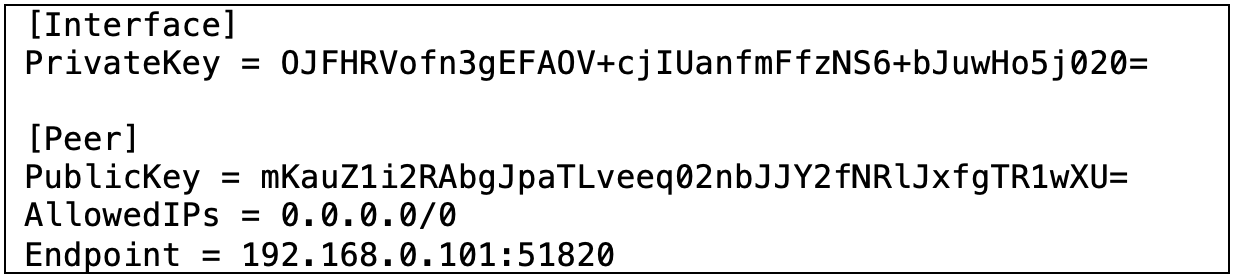
\includegraphics[width=8cm]{paper/images/wg_conf_std.png}
\caption{example WireGuard configuration file from the reference implementation}
\label{fig:wg_config}
\end{figure}

\begin{figure}[ht]
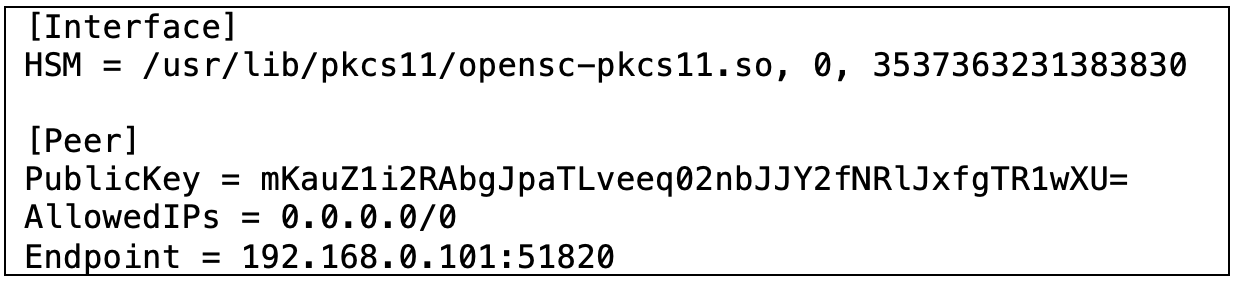
\includegraphics[width=8cm]{paper/images/wg_conf_hsm.png}
\caption{example WireGuard-HSM configuration file}
\label{fig:hsm_config}
\end{figure}
This modification removes the requirement for defining and storing the private-key in the plain-text file. The HSM directive tells the program two, and optionally three things. First it lists the PKCS\#11 library path. Second, the slot id  to use on the security key. Thirdly and optionally, the pin required to access the slot.

The detailed workings of the PKCS\#11 interface are out of scope for this paper, however it suffices to say that for interfacing with a security-key, PKCS\#11 requires a slot ID and a secret pin-number for that slot, to enable privileged operations like key-signing or key derivation. The PKCS\#11 interface will inform the caller if they successfully logged into the slot and if the requested operation succeeded or not.

Security is a balancing act between overall system security and user-convenience. Making a system more secure can often come at expense of user-convenience. After writing the initial version of pkclient, I added in the functionality to give the user a choice in saving the pin-number in the configuration or omit it entirely. When the pin is omitted and the configuration file is read to WireGuard-HSM, the program will prompt the user for the pin before the WireGuard interface is configured. If pkclient doesn't have the pin number for the given slot, it cannot be sure the hardware security key is configured properly. Saving the security-key pin-number in the configuration file reduces the security of our system a little and I point this out in the threat model. 

TODO Finish this section?



\section {Methodology}
I will perform a comparative threat model analysis of the reference implementation and WireGuard-HSM. This analysis will show the relative strengths and weaknesses of the designs and what I have improved on.

I will also use some traditional software metrics to evaluate the project.

\chapter {Evaluation}
\section{Threat models analysis}

\subsection {WireGuard - Reference Implementation}
\label{section:tm}


Here I present my analysis of the reference implementation of WireGuard. This threat model is focused on WireGuard's asset handling related to the private key, the security controls around it and the threat actors that could be lurking on the system. This computer running WireGuard will be considered Alice's computer and the WireGuard peer Alice connects to is Bob. Alice's computer has been turned on but Alice has not yet established a WireGuard session to Bob's computer. Refer to section \ref{handshake_message} on how WireGuard establishes a peer session. 

\begin{figure}[ht]
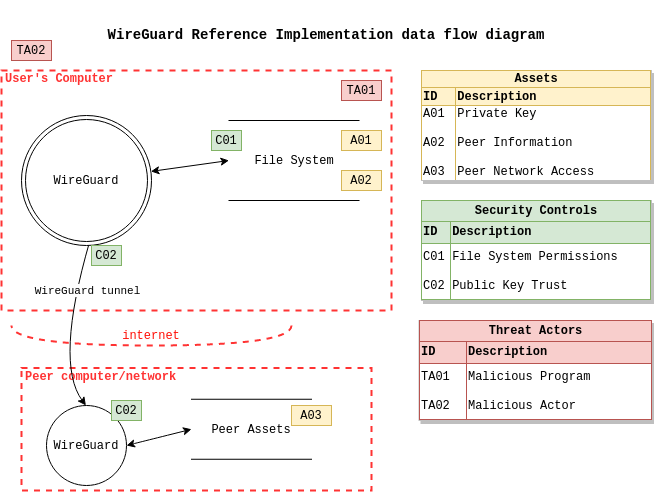
\includegraphics[width=14cm]{paper/images/WG_DFD.drawio.png}
\caption{A threat model for the WireGuard reference implementation - data flow diagram}
\label{fig:wg_ref_dfd}
\end{figure}


The file system on Alice's computer contains the WireGuard configuration file \ref{fig:wg_config}. 
Asset A01 is Alice's Curve25519 static private key. Asset A02 is Bob's connection information consisting of his Curve25519 static public key and DNS address. It is important to note that in this threat model, both of these assets reside in the same location. Access to the configuration file gives access to both assets.

The primary source of access control in WireGuard's reference implementation for A01 and A02 is C01: proper file system permissions. Most of the documentations (TODO CONFIRM) indicate that the permissions should be set on the WireGuard configuration file to allow only administrator access and restrict access by unprivileged users. For most of the reference implementations that I can find, this is not an enforced measure, meaning WireGuard will still start and not complain if the configuration file permissions are insufficient. 

\section{Threat Actor 1}
Let us consider our primary threat, TA01: a piece of malware that has gained access to Alice's computer by some means. A plausible infection scenario might be that the malware has been delivered to Alice's machine via a compromised website advertisement that is exploiting a new web-browser vulnerability in order to escape the web-browser protections and read files on the local machine.  This malware has been programmed to look for and harvest assets on infected hosts. In our case it will look for common filenames or patterns within files that look like WireGuard configuration files.  
\subsection{insufficient permissions}
If TA01 gains read-only access a single time to Alice's computer and the file system permissions were not correctly set on the WireGuard configuration file, then the malware gains access to A01 and A02. Access to these assets results in loss of A03 by bypassing C02. See section \ref{impersonation} to see how this works.

\subsection{sufficient permissions}
If C01 is configured properly, then TA01 will have a more difficult time gaining access to A01 and A02. This offers a single layer of security so TA01 will need to perform a pivot in order to bypass the security control C01. Exploit chains are common-place in today's security field so let's consider an attack that uses more than one vulnerability. Now that TA01 has access to Alice's computer, it will need to pivot in order to bypass C01. I will present three different areas of attack that could be used to pivot. Chain an exploit which results in one of the following: gaining administrative privileges, modify file system permissions, trick a privileged process into disclosing the file contents. This is not an exhaustive list of pivots but these three are reasonable scenarios. Once any single one of these pivots is performed, then TA01 has access to A01 and A02 which results in loss of A03 by bypassing C02.

\section{Threat Actor 2}
Our second threat actor is a malicious user who gains direct or indirect access to Alice's computer. 

Let us consider the in-direct method first since it's very common-place. This could be performed by this threat actor using social engineering tactics such as a phone-call masquerading as someone from Alice's IT department, asking her to in some way disclose the contents of the WireGuard configuration file, leading to disclosure of assets A01 and A02.

In a direct method of attack, the second threat actor gains physical access to Alice's laptop and uses some technical or non-technical exploit to read the hard-drive. A technical exploit might be a disk-encryption key recovery vulnerability, allowing TA02 access to the hard drive. TODO expand on this section
\subsection{off-line access}
If Alice's laptop is not protected by hard-drive encryption, then it is trivial for an attacker who has physical access to a laptop to mount and read the contents of the file system on the target device, leading to loss of A01 and A02.

\section{Vulnerabilities}
Once any of the previously described weaknesses and have been taken advantage of by a threat, and the threat actor gains access to assets A01 and A02, this creates two different vulnerabilities in our WireGuard system for Alice and Bob. TODO (define CIA Triad earlier and define impersonation and DOS)
\subsection{impersonation}
\label{impersonation}
In order to perform a WireGuard handshake as Alice, all a threat actor needs is Alice's private key (A01) and Bob's public key (A02). With these two pieces of information, a threat can now effectively impersonate Alice from any computer in the world, almost undetected. I discuss the situation in which the attack is detected in the next section \ref{dos}. Loss of A01 and A02 allows for bypassing the public key trust in C02, for any peer found in the configuration file, which is A02. This gives the threat actor access to any assets that are held on Bob's computer or network. VPN's are commonly used as the first layer of defense for network access, so A03 could be access to a network resource that is hidden behind the WireGuard VPN. It is reasonable to assume this attack could also be the first step in an exploit chain to gain access to more assets. 

\subsection{Denial-of-Service}
\label{dos}
If asset disclosure is not the goal of an attacker then denial of service is a viable threat to consider. Once a threat can perform impersonation, that can be used to perform a denial of service attack against Alice's WireGuard connection to Bob. When Bob receives and establishes a handshake with Alice's credentials, the initiator established that handshake with a 'sender's index'. This index is a randomly generated 4-byte value which the peer uses to identify the sessions. Once Bob has an established session with Alice's credentials, it will drop any handshake initiations messages that don't contain that index value. In this situation the attacker simply needs to establish a connection before the real Alice does, and Alice will be unable to perform a handshake with Bob until the attacker disconnects.

This denial of service attack would not be noticed by Bob because his WireGuard process thinks he has a legitimate session established with Alice and will silently drop other connection attempts. Alice would only notice that she is unable to establish a session with Bob. Alice would have to communicate with Bob via alternative means, and have him look at his computer's WireGuard session output, then they would need to note that Alice's session is currently established and what remote IP has established the session.

===================================


\section{WireGuard-HSM Threat model}
Here I present my threat model analysis of the WireGuard-HSM. This threat model is also focused on WireGuard-HSM's asset handling related to the private key and peer public keys, the security controls around them and possible threat actors to the system. The computer running WireGuard will be considered Alice's computer and the WireGuard peer Alice connects to is referred to as Bob. Alice's computer has been turned on but Alice has not yet established a WireGuard session to Bob's computer. Refer to section \ref{handshake_message} on how WireGuard establishes a peer session. 


\begin{figure}[ht]
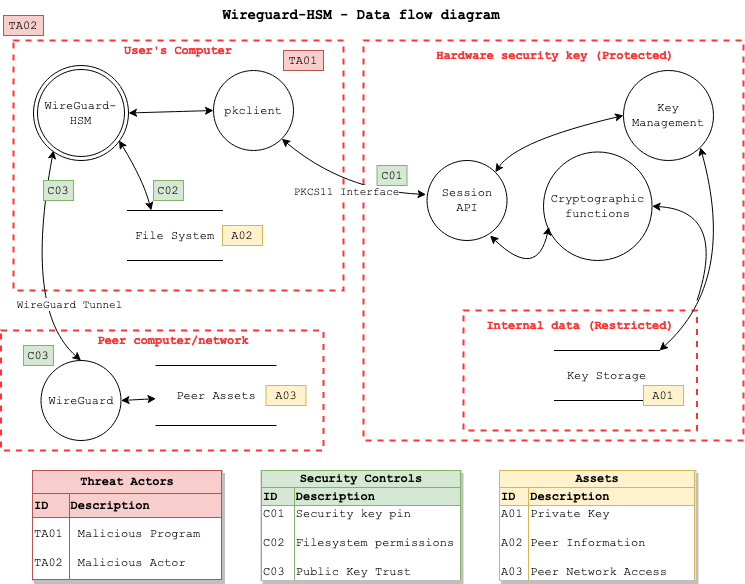
\includegraphics[width=14cm]{paper/images/WGHSM_DFD.drawio.png}
\caption{A threat model for WireGuard-HSM - data flow diagram}
\label{fig:wg_hsm_dfd}
\end{figure}

\subsection{Threat Actor 1}
Let us consider our primary threat, TA01: a piece of malware that has gained access to Alice's computer by some means. A plausible infection scenario might be that the malware has been delivered to Alice's machine via a compromised website advertisement that is exploiting a new web-browser vulnerability in order to escape the web-browser protections and read files on the local machine.  This malware has been programmed to look for and harvest assets on infected hosts. In our case it will look for common filenames or patterns within files that look like WireGuard configuration files.  

\subsection{insufficient permissions}
If TA01 gains read-only access a single time to Alice's computer and the file system permissions were not correctly set on the WireGuard configuration file, then the malware gains access only to A02. Access to these assets results in loss of A03 by bypassing C02. See section \ref{impersonation} to see how this works.

\subsection{sufficient permissions}
If C01 is configured properly, then TA01 will have a more difficult time gaining access to A01 and A02. This offers a single layer of security so TA01 will need to perform a pivot in order to bypass the security control C01. Exploit chains are common-place in today's security field so let's consider an attack that uses more than one vulnerability. Now that TA01 has access to Alice's computer, it will need to pivot in order to bypass C01. I will present three different areas of attack that could be used to pivot. Chain an exploit which results in one of the following: gaining administrative privileges, modify file system permissions, trick a privileged process into disclosing the file contents. This is not an exhaustive list of pivots but these three are reasonable scenarios. Once any single one of these pivots is performed, then TA01 has access to A01 and A02 which results in loss of A03 by bypassing C02.

== NEEDED? ==
The secrecy of a client's private key is paramount to proper client identification and authorization in WireGuard. WireGuard's design protects many aspects of the key handling that have been error prone in past VPN designs (TODO )
My threat model is based around the secrecy of the private key and reducing the risk found in the reference implementation of WireGuard. Since WireGuard allows clients protected-access to resources across networks, there is value for an attacker to desire access. 
There are two main threats to this privacy.  malware infecting a computer running the reference implementation of WireGuard. The malware could be resident on the computer or it could be a single instance where a browser exploit allows an arbitrary file to be read. Our guards against malware that runs on user's computer and gains access to the plain-text configuration file for WireGuard, leaking the private key which gives the bad-actors the ability to connect to the configured wireguard-peers undetected, as the legitimate user.
== /NEEDED? ==



\section{software metrics}

\subsection{performance}
WireGuard-HSM makes use of a USB connected security key. The cryptographic function to derive a shared key is now locked behind a small embedded device that is much less powerful than the computer running it. I wanted to see what performance impacts my design might introduce to the system.

In order to benchmark the performance of the implementations, I added a timing function that saves the current time at the beginning of the sharedSecret() function in WireGuard and DeriveNoise() in pkclient. The print statement that indicates how long the call took is deferred, meaning  once the surrounding function returns, the deferred function executes. 
The sharedSecret() function is responsible for taking a public key as input and deriving a shared secret key. The sharedSecret() is a function of a private-key object.

WireGuard-HSM will still make use of sharedSecret() but only after generating the ephemeral session keys. 


\chapter {Discussion of Results}
\section {Introduction}
I will discuss the limitations of my project as well as the technical hurdles that I faced while implementing and evaluating my project.

\section{program authentication}
One limitation of WireGuard and WireGuard-HSM that can be understood looking at the threat model is that WireGuard operates at the network level, acting as virtual network interface, it makes no guarantees at the operating system level about who or what application is allowed access to the tunnel or not. It is understandable that to maintain platform independence, this is not a goal of the WireGuard project but researchers have proposed a modified WireGuard client that authenticates each application on a smartphone, that is given access to the WireGuard virtual tunnel interface. A major downside of this proposed modification is it requires the user to enter their pin number separately for each application that requires tunnel access, every time WireGuard is started.\cite{wu_sewg_2020}

\section {Limitations}
I had initially hoped that my project could include mobile operating systems such as a smart phone. Users can easily use security keys with mobile operating systems but due to the limited support for X25519 among hardware security keys, this didn't make sense at the time of writing. The Nitrokey Start connects only via USB-A port is absent from most smart-phones. Connecting the Nitrokey Start to a smart phone would require a converter and then

2\textsuperscript{60} messages are exchanged.


\chapter {Conclusion and future work}

\section {Future Work}
There are several areas where I would like to improve WireGuard-HSM that have been identified over the course of implementing and evaluating the system. These areas include pin handling and security key availability. 

\subsection{pin handling}
 A user may choose not a save the security-key pin in the WireGuard-HSM configuration file. In this mode, the program must prompt user for the pin. Currently this prompt is very simple and given on the command-line when the user runs WireGuard-HSM. This prompt is easy to miss and wouldn't work very well if WireGuard-HSM was implemented as a kernel module. A better approach would be to have the prompt implemented as a system-dialog window, that appears over any existing windows, making very simple for the user to omit the pin and only enter it when using WireGuard-HSM. Finding a Go-module that opens window dialogues and supports multiple operating system was deemed out of scope for this project but it will be my next addition to the program since it would increase the ease-of-use for the program. 
 
\subsection{security key diversity}
Hardware security-key support for curve25519 and specifically X25519 is, as of writing, very limited. Nitrokey 3 is planned to support X25519 but the hardware is still not in mass production. I would like to see bio-metric hardware-keys with X25519 support, this would add an additional layer of security to our model as it further authenticates the user. As of writing, I could find no planned development for such a key. Many hardware-security keys have introduced support for near-field-communication (NFC) which makes using them with mobile devices almost seamless. Having a security-key with Curve25519 support, would make integrating WireGuard-HSM with mobiles devices easier and put less burden on the user. 

\subsection{kernel-mode support}
WireGuard-HSM is written using the Go language version of Wireguard but a kernel-mode version would be more practical. The Go-version of WireGuard warns users on start-up that if they are on a supported operating system, the kernel version has better support and offers better performance. The main challenge in writing the kernel mode version will be the PKCS\#11 integration and handling user interaction between a kernel module. A small program like pkclient that handled the PKCS\#11 integration and user prompts, would be a good start. 

\section {Time Table}
\begin{center}
\begin{tabular}{ |c|c| } 
 \hline
Week & Task \\
 \hline
March 13th & Threat Model DFD and Paper work \\ 
  \hline
March 20th & Continue work on threat model analyis. Write project background section \\ 
  \hline
March 27th & Finish project background discussion and edit it. 
cont comparative analysis of designs   \\  
 \hline
April 3rd & Feedback and polishing threat model section  \\  
 \hline
April 10th & Generate graphs and continue analysis. Go/no-go for defense schedule  \\  
 \hline
April 17th & Ask committee for defense dates. Formal analysis work if possible \\  
 \hline
April 24th & Meet and discuss state of paper and project. Formal analysis work cont  \\  
 \hline
May 1st  & If good: start presentation writing  \\  
 \hline
May 8th  & continue presentation writing. Formal analyse done and integrated into paper  \\  
 \hline
May 15th  & continue presentation writing   \\  
 \hline
May 22nd  & Ideal week for defense. Write last-minute changes  \\  
 \hline
May 29th  & Integrate feedback from defense into paper  \\  
 \hline
June 5th  & Integrate feedback from defense into paper part 2. 
Submit final paper \\  
 \hline
 
\end{tabular}
\end{center}

\bibliographystyle{plain}
\bibliography{references}
\end{document}
